% 
\documentclass[a4paper,10pt]{article}
\usepackage{a4wide}
\usepackage[utf8]{inputenc}
\usepackage[usenames, dvipsnames]{color}
\usepackage{titlesec}
\usepackage{graphicx}
\usepackage{wrapfig}
\usepackage[textsize=tiny]{todonotes}
\usepackage{hyperref}
\usepackage{multicol}
%\usepackage{lipsum}
\titleformat{\section}
{\color{blue}\normalfont\Large\bfseries}
{\color{blue}\thesection}{1em}{}
\titleformat{\subsection}
{\color{cyan}\normalfont\large\bfseries}
{\color{cyan}\thesubsection}{1em}{}
\titleformat{\subsubsection}
{\color{blue}\normalfont\small\bfseries}
{\color{blue}\thesubsubsection}{1em}{}
\usepackage[font=footnotesize,labelfont=bf]{caption}
\usepackage[toc]{multitoc}
\renewcommand*{\multicolumntoc}{2}
\setlength{\columnseprule}{0.5pt}
\newcounter{save}
\title{Data Science and Computational Science - report from a committee at the Faculty of Mathematics and Natural Sciences, University of Oslo}
\author{Leader: Geir Dahl (MI)}
\date{
\begin{tabular}{cc}
Anne Solberg (IFI)& Ole Christian Lingjærde (IFI)\\  
Morten Hjorth-Jensen (FI)&  Heidi Sandaker (FI)\\  
Ingrid Glad (MI)&  Geir Storvik (MI)\\

\includegraphics[width=0.4\textwidth,trim={0cm 0cm 0cm 0cm},clip]{datascience-630x180.jpg}&
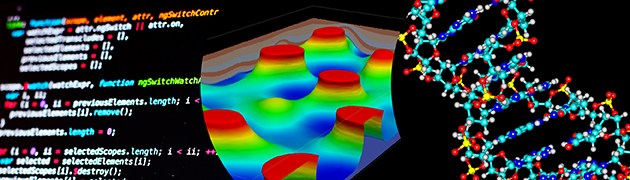
\includegraphics[width=0.4\textwidth,trim={0cm 0cm 0cm 0cm},clip]{computerscience-630x180.jpg}
\end{tabular}
}
\setlength\parindent{0.3cm}
\begin{document}

\maketitle
%\begin{multicols}{2}
{\small
  \tableofcontents
  }
%\end{multicols}

\section{Computing Across  Disciplines: How the University of Oslo  should meet the Future}

Data Science (DS), including machine learning, and Computational Science (CS) are fast-growing scientific areas of high importance  for the Faculty of Mathematics and Natural Sciences.\footnote{
The age of analytics: Competing in a data-driven world \url{https://www.mckinsey.com/business-functions/mckinsey-analytics/our-insights/the-age-of-analytics-competing-in-a-data-driven-world} and
\url{
https://www.mckinsey.com/business-functions/digital-mckinsey/our-insights/big-data-the-next-frontier-for-innovation}}

Data Science and Computational Science play a central role in scientific investigations in general and are central to innovation in most domains of our lives. They underpin the majority of today's technological, economic and societal feats. We have entered an era in which huge amounts of data offer enormous opportunities, but only to those who are able to harness them. It is  expected that a large majority  of jobs in the STEM (Science, Technology, Engineering and Mathematics) fields will require skills and competences that involve  computing.
Furthermore, the 3rd Industrial Revolution will alter significantly the demands on the workforce. To adapt a highly-qualified workforce to coming challenges requires strong fundamental bases in STEM fields. Data Science and Computational Science can provide such bases at all stages. 
These developments, needs and future challenges, will play an essential role in shaping future technological developments. Most of these developments require true cross-disciplinary approaches.
There is a massive interest in society, and in the job market,  for candidates with this kind of DS and CS background. In particular, the interest concerning machine learning techniques is noteworthy.  

{\bf This document aims at developing strategies for meeting these future challenges. One important step in order to meet the future, is the hiring of new researchers and faculty with the competences and skills which are needed in order to harness the many new possibilities, as well as developing new research and educational strategies that can serve our society at large. There are several possible ways to meet these challenges. The present document focuses on the establishment of a new   center (DASCO) on Data Science and Computational Science.}



\subsection{Background}
In the fall of 2018 the University of Oslo started two new Master of Science  programs in Data Science and Computational Science at the University of Oslo, and the first students are now enrolled. There was a major interest for each of these Master of Science programs with many applicants from Norway and abroad. Moreover, there is  a  broad interest for CS  and DS courses 
across study programs at the Faculty of Mathematics and Natural Sciences (FMNS) at the University of Oslo (UiO). This applies to other Faculties/colleges and disciplines as well. There is a growing interest in for example Machine Learning in a wide range of fields, from Economics to Political Science and Psychology. 

A survey conducted during the fall 2018 shows that the use of Data Science and Computational Science tools form important parts of the research performed at all departments of the FMNS, see Figure~\ref{fig:dept}.\todo{IG: Feil ref. Er i Appendix 3} Some of the respondents state they only require off-the-shelf tools while many others are involved in so large and complex problems that cutting-edge methodology has to be applied, or even developed. Pure methodological research within DS and CS is mainly concentrated at the departments of Informatics (IFI) and Mathematics (MI). Workshops and seminars have on several occasions been organized within and outside the FMNS. A common feedback from these activities is the need for a forum for scientific discussions and collaborations on DS and CS topics.


The Faculty of Mathematics and Natural Sciences at UiO has recently presented its strategic plan for the period till 2030, with several ambitious proposals and strategic themes.  One of these strategic themes is \emph{digitalization and computational science}, where Data Science and Computational Science are expected to play a central role. 
The University of Oslo has in all of the STEM fields strong research and educational activities within DS and CS, with excellent opportunities for further strengthening our activities in Data Science and Computational Science. We list some of these activities here:
\begin{itemize}
\item The Faculty of Mathematics and Natural Sciences has several Centers of excellence in research and innovation as well as excellent research groups where Data Science and Computational Science play a major role.
\item There is a  newly established center of excellence in educational research, the Center of Computing in Science Education.
\item Newly established Master of Science programs in Data Science and Computational Science.
\item Computational topics are included in all undergraduate STEM programs.
\item Strong links with research laboratories like SINTEF, SIMULA and the Norwegian Computing Center (NR).
\item Involvement of other initiatives like Startup-Lab, NORA etc. Furthermore the contact with industry is strong, and the Akademia agreement between the FMNS and Equinor provides support to positions and activities in Data Science/Machine learning.
\end{itemize}
With a close coordination between the departments of Mathematics,  Informatics as well as other involved departments at the Faculty of Mathematics and Natural Sciences, we have the possibility to  position UiO as a leading institution internationally (and as a national leader) within Data Science and Computational Science. Furthermore, UiO has the potential to develop cross-college educational programs in Data Science and Computational Science, from undergraduate programs to graduate programs that will serve the needs of both the public sector and the private sector. 

The Faculty of Mathematics and Natural Sciences at UiO has appointed a committee whose task is to provide recommendations concerning the activities in the DS and CS areas. The main focus of the committee has been on the mathematical foundations of Data Science and Computational Science, including statistics, machine learning and computations. However, the committee was also tasked with covering  more application-oriented activities %(for example machine learning) 
and the crucial connection between research focused on methods  and research focused on applications. A detailed description of the mandate can be found in Appendix~\ref{ap:mandat}. 




In the discussions here we define Data Science as the whole process of discovery, knowledge extraction and decision making based on data.
Computational science  is a rapidly growing multidisciplinary field that uses advanced computing capabilities to understand and solve complex problems. It is an area of science which spans many disciplines, but at its core it involves the development of models and simulations to understand natural systems. In practical use, it consists  typically applications of computer simulations and other forms of computations from numerical analysis and theoretical computer science to solve problems in various scientific disciplines

There is a clear tendency that methods and techniques from both DS and CS play a central role in  studies of present and future scientific problems.  Both DS and CS have mathematics and informatics as a common basis. Moreover, statistics and statistical data analysis  play central roles in many DS and CS applications and studies.  Computing has
also become one (of several) important ingredients in DS, in particular  within deep
learning for applications in computer vision where efficient hardware and GPU implementations
are  essential. The  exciting   field  of  Machine  Learning  is  perhaps  one  of  the  best  examples
where algorithms and methods from DS and CS are used with great success.  As an example, optimization algorithms play an important role in practically  all deep learning algorithms in supervised and unsupervised machine learning. 

A central question is thus: 
How should the activities in DS and CS be organized at the Faculty of Mathematics and Natural Sciences in order to maximize the benefit in terms of fruitful scientific collaboration and impact, and provide attractive study programs as well?


\section{Vision and actions}

In order to answer the above questions, 
this document aims at developing strategies for meeting  present and future challenges in Data Science  and Computational Science at UiO, both from a research perspective and an educational perspective. To accomplish this we propose\newline 

{\bf \em to establish a center in  Data Science and Computational Science at the Faculty of Mathematics and Natural Sciences of the University of Oslo. The center aims at becoming the national leader in Data Science and Computational Science and is expected to become an internationally acknowledged hub for research and education in these fields.}




\subsection{Main goals}
\begin{enumerate}
\item The establishment  of DASCO, a highly visible  national and international center for {\bf Data Science and Computing}. 
\item A physically co-located center for Data Science and Computational Science researchers from the Faculty of Mathematics and Natural Sciences. The center will also strive to open up for research and applications of DS and CS in disciplines outside the traditional realm of Mathematics and Natural Science.  
\item A hub/node policy (Figure~\ref{fig:dept1}): The center with its researchers will spearhead new developments in Data Science and Computational Science. It will  provide the physical meeting places for DS and CS activities at UiO, ranging from collaborative research programs to the organization of seminars and workshops and new educational programs in DS and CS. It will act as the main hub for all DS and CS related activities. The various nodes in the figure below represent  related activities at the different departments of the FMNS as well as other disciplines and Faculties at the University of Oslo. 
\item The new center will strengthen  existing collaborations as well as opening up for new  collaborations in Data Science and Computational Science across disciplines.  
\end{enumerate}

The center will be a joint venture  between the departments of Informatics and Mathematics. These two departments represent the main contributors to the center and together with domain specialists from other departments at the FMNS, the aim is to strengthen DS and CS at the University of Oslo.
The new center will be unique among computational academic units nationally, the first to comprehensively treat computation as the triple point of algorithm development and analysis, high performance computing, and disciplinary knowledge with applications to scientific modeling and data science. The center recognizes computation as a new discipline rather than decomposed into isolated sub-disciplines, enabling application-driven computational modeling and data-driven discoveries, while also exposing disciplinary scientists  to advanced tools and techniques, which will ignite new transformational connections in research and education. This research nexus also gives rise to the educational opportunities driven by similar synergy, leveraging common resources among disciplines, and enabling joint programs and unique degrees across disciplines. The overall goal of this center is to bring together faculty and researchers who combine the most important aspects of computation and disciplinary research, thus enabling cutting-edge interdisciplinary science and the training of both undergraduate and graduate students.

 Such a center will have a strong national and international visibility, a feature which is important for recruiting students as well as for  connections with external partners from the public and the private sectors. We foresee that this center will develop a long-term perspective, where a central aim is to oversee and adjust  to new developments in the broad areas of Data Science, Computational Science and Scientific Computing.



\begin{wrapfigure}{R}{0.4\textwidth}
\centering
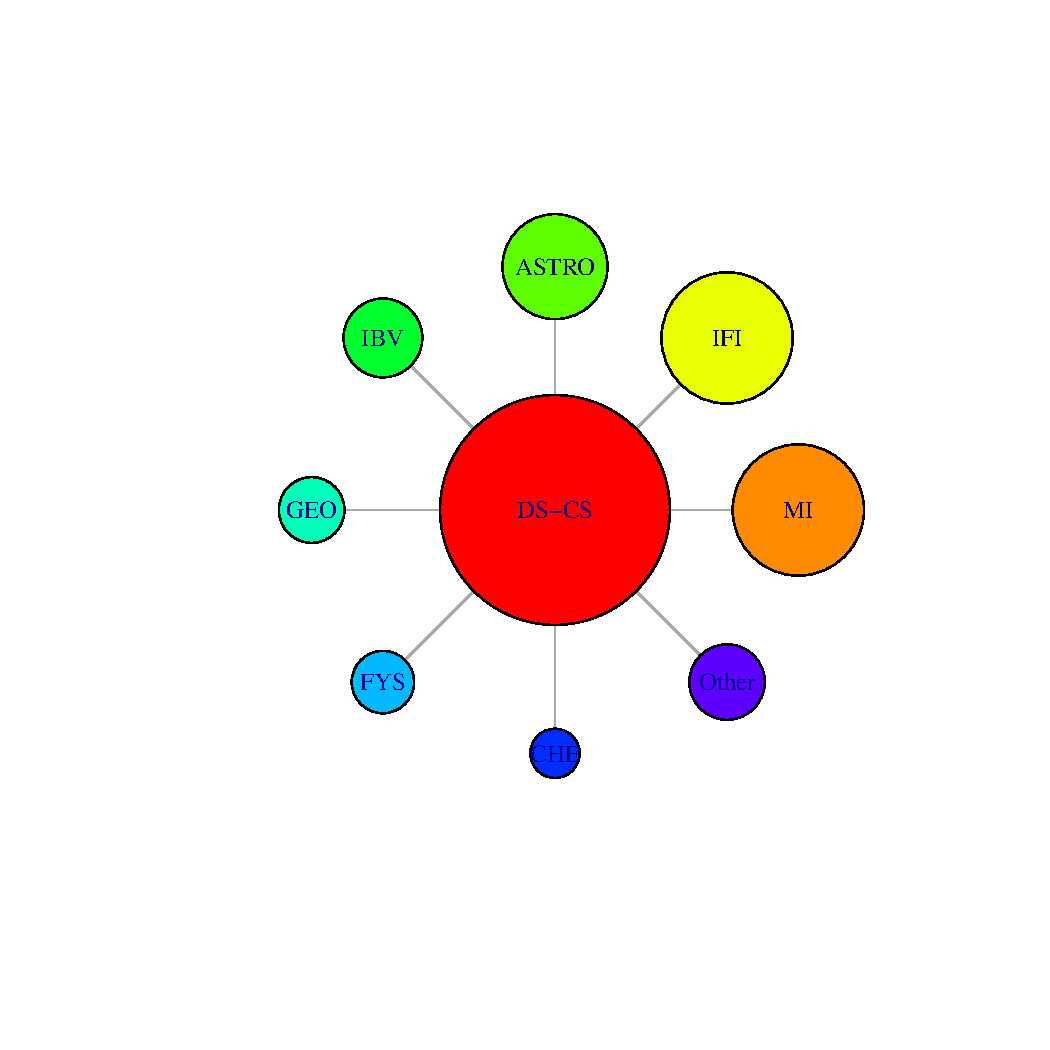
\includegraphics[width=0.4\textwidth,trim={2.4cm 4.4cm 1.8cm 3.64cm},clip]{Hub_node.pdf}
\caption{\label{fig:dept1}The Hub-node structure. The sizes of the nodes corresponds to responses from a survey of interest in CS or DS at the FMNS during the  fall semester of 2018.}
\end{wrapfigure}
%\lipsum[1-6]

This organization upholds the basic and classical disciplines behind DS and CS as well as  opening up for incorporating  new developments. It aims at connecting the different departments in a totally new way, and will stimulate interdisciplinary research significantly. The collaboration between the departments of Informatics and Mathematics is crucial since both departments have several strong groups in machine learning/Data Science. Both departments consider this as a strategic area of research and education. Moreover, Mathematics and Informatics are central topics in both Data Science and Computational science. Together with domain specialists with strong interest in CS and DS at other departments at the Faculty of Mathematics and Natural Sciences, the center will include and integrate interested representatives from other departments  in the best possible way. We envision that the center will be a truly interdisciplinary unit that strives to focus on algorithmic science and its applications to a range of critical research topics. The center will thus consist of  faculty from the departments of Informatics and Mathematics as well as disciplinary scientists from other departments. 




\subsection{Subgoals}

\begin{enumerate} 
\item Develop internationally leading research groups in Computational Science and Data Science
\item Develop excellence in both application driven and methodological research.
\item Be an important contributor to the Faculty of Mathematics and Natural Sciences' strategic plan for digitalization and computing. 
\item Develop top international level educational programs and learning environments in Data Science and Computational Science.
\item Be a driving force in the education of the next generation of school teachers and university teachers, with a strong focus on digital competences.
\item Attract researchers and students of highest quality.
\item Develop new initiatives in Computational Science and Data Science
\item Attract extensive external funding, both from industry/public sector and research councils,  with the vision of establishing a new center of excellence.
\end{enumerate}



\subsection{Proposal}
To achieve these goals, we propose the following:
\begin{enumerate}
\item Structure of the center
\begin{itemize}
\item Recruit a  scientifically strong leadership team able to coordinate research activities and to create good scientific interactions between researchers from different disciplines and backgrounds. 
\item A core group or researchers working most of their time at the center combined with domain-experts with joint positions, e.g. 20\% at DASCO and 80\% at their ``home'' departments.
\item A scientific advisory board with international members.
\item A small administrative staff, including a person responsible for administrative tasks related to teaching.
\end{itemize}
\item New positions
\begin{itemize}
\item At least {\bf ten} new permanent positions with a strong methodological orientation as well as  having a connection/responsibility towards a specific discipline/domain.
\item 15-20 PhD/Postdocs with joint supervisors to encourage interdisciplinary activities.
\end{itemize}
\item Educational responsibility:
\begin{itemize}
\item Establish a Graduate programs in DS and CS.
\item Develop and supervise courses in DS and CS for Master of Science programs in other disciplines.
\item Offer continuing education courses (including possibly certificates) in DS and CS.
\item Develop courses, and course modules in Data Science and Computational Science to be included in various bachelor programs. 
\item Develop a common bachelor program  in Data Science and Computational science.
\item Develop close collaborations with the Center for Computing in Science Education (CCSE) 
\end{itemize}
\item Develop formal affiliations and responsibilities to "home" departments, with  responsibilities through agreements delegated to the center. 
\end{enumerate}

A DS and CS center will gain high visibility and facilitate
connections to the public and private sectors, with the aim to
strengthen links to industry, research institutes and society in
general.  In our proposal we suggest not only to integrate researchers
within each of the separate fields of DS and CS but also to integrate
these fields. Although being separate fields with different focus,
"users" typically need both and there is also much methodological
overlap making a "convergence" of these fields a possible benefit for
all parts. For students, the differences between these fields are
sometimes difficult to understand, making thereby a common profile
more meaningful.


A central element in addressing the above needs and challenges is the
hiring of new faculty members and researchers. We recommend a model
where new positions (faculty and researchers, permanent and/or
temporary) are earmarked for the departments of Mathematics and
Informatics in order to develop new research and educational
directions in Data Science and Computational Science.  The new faculty
will thus be tasked with developing new research and educational
programs in Data Science and Computational Science. It is essential
that the hired faculty can/should have shared positions with existing
departments (for example a 70\% position at say Mathematics or
Informatics and 30\% at the department of Physics), similarly, faculty
with a computational profile and interest at existing departments can
have shared positions at the Department of Mathematics and the
Department of Informatics. The shared positions entail also sharing of
teaching obligations. This will ensure transfer of knowledge as well
as the establishment of new and cross-disciplinary research and
oversee the development of new educational programs and efforts.

We suggest a small administrative staff associated with DASCO with
responsibilities associated with study programs, organizing
seminars/courses and industrial contacts (research collaboration,
student internships).

The proposed organization will also influence our study programs.  The
creation of a coherent set of undergraduate and graduate degrees, with
accompanying courses, supports two complementary goals. First, a
coherent program will allow the University of Oslo to consolidate
undergraduate and graduate training in data analysis and computations
in the STEM fields as well as introducing such tools to other
disciplines, reducing redundancy in the courses taught and allowing
the university to offer a wider range of more specialized advanced
courses. Second, we will create a set of degrees that are designed to
give our students a strong introduction to data science and computing
that will complement UiO’s existing disciplinary training, and which
will make them better suited to be a part of the workforce in the 21st
century. Finally it will enable our students to develop and use Data
Science and Computational Science across the disciplines.  One desired
result of the creation of these courses and programs is the foundation
of a strong community of students from different disciplines that use
similar techniques to solve a wide range of problems, which will
promote broad, interdisciplinary thinking and will help to raise the
visibility of data science and computing across disciplines.  We note
that an extra benefit of these educational efforts is that UiO will
become an ideal place to perform research in data science and
computational science education, a topic of critical importance that
has thus far received less attention. We foresee strong links with the
recently established Center for Computing in Science Education.

The Faculty of Mathematics and Natural Sciences has over the last 15
years integrated computational science topics in our bachelor
programs. It is now time to integrate data science as well into our
bachelor programs. As of now, this is only partly done through some
“practical” introductory courses in statistics and domain specific
courses which include selected aspects of data analysis. What we in
particular need is an introduction to basic knowledge about using the
“scientific method" (the empirical method of knowledge acquisition)
including representability of data for the problem at hand, design of
data collection, the bias-variance trade-off, as well as principles
for evaluating the quality of the obtained results.

In addition, the center should strive to establish interdisciplinary
projects and have close collaboration with similar international
centers.  Integrating the development of computational infrastructure
at USIT into the center is also an important aspect.


These efforts will open new avenues for research, will enable UiO to
compete and propose new center-level funding opportunities as well as
totally new research areas (in the Humanities, for example) in
computation and data-driven related areas that are currently beyond
our reach. It will facilitate the training of scientists and students
to be an effective 21st century workforce. It will also develop
courses on modern computational techniques and data modeling that meet
the needs of society, both for the public and the private sector.





\subsection{Members}
\begin{itemize}
\item Defining the core group: There are potentially many groups and individual researchers that would like to be involved in such a center. The center needs a clear definition of the main focus. One possibility is a generic but problem-motivated approach. More specifically, a core group can then involve (with estimated numbers in parenthesis)
several “primary” members from MI, IFI and  other departments (f.ex. Physics, Chemistry, Biosciences, Geosciences and Astrophysics), with joint positions with say a 80/20 share(80\% at DASCO and 20\% at another department), while some positions may be fully allocated  (100\%) to the center:
\begin{itemize}
\item the whole section of Statistics and Data Science at MI, (8 permanent faculty) and possibly some individuals from the risk analysis, mechanics and PDE groups (5-6).
\item Several individuals from different sections at IFI, Biomedical informatics (3), Digital signal processing and image analysis (4), Language Technology (1-2), Robotics and intelligent systems (?), and Analytical solutions \& reasoning (?)
\item The Computational Physics group at the Department of Physics (2) and possibly representatives from other groups, such as experimental particle physics where applications of DS play a  large role.
\end{itemize}
\item Several faculty members from other  departments of the FMNS, organized as joint positions of the type 20/80 or other fractions, such as e.g. 20\% time at DASCO and 80\% time at Astrophysics, Chemistry, or any other MN department. This is a recommended position for researchers that have a significant  focus on DS+CS in their work, but their main activity remains  at their host department. These researchers will be a part of the methodological focus of DASCO, and will contribute with and discuss interesting challenges that arise in different applications. Note: The 80/20 split concerns both research and teaching responsibilities. 
\end{itemize}


\subsection{Topics}


\begin{wrapfigure}{r}{0.4\textwidth}
\centering
\vspace*{-0.5cm}
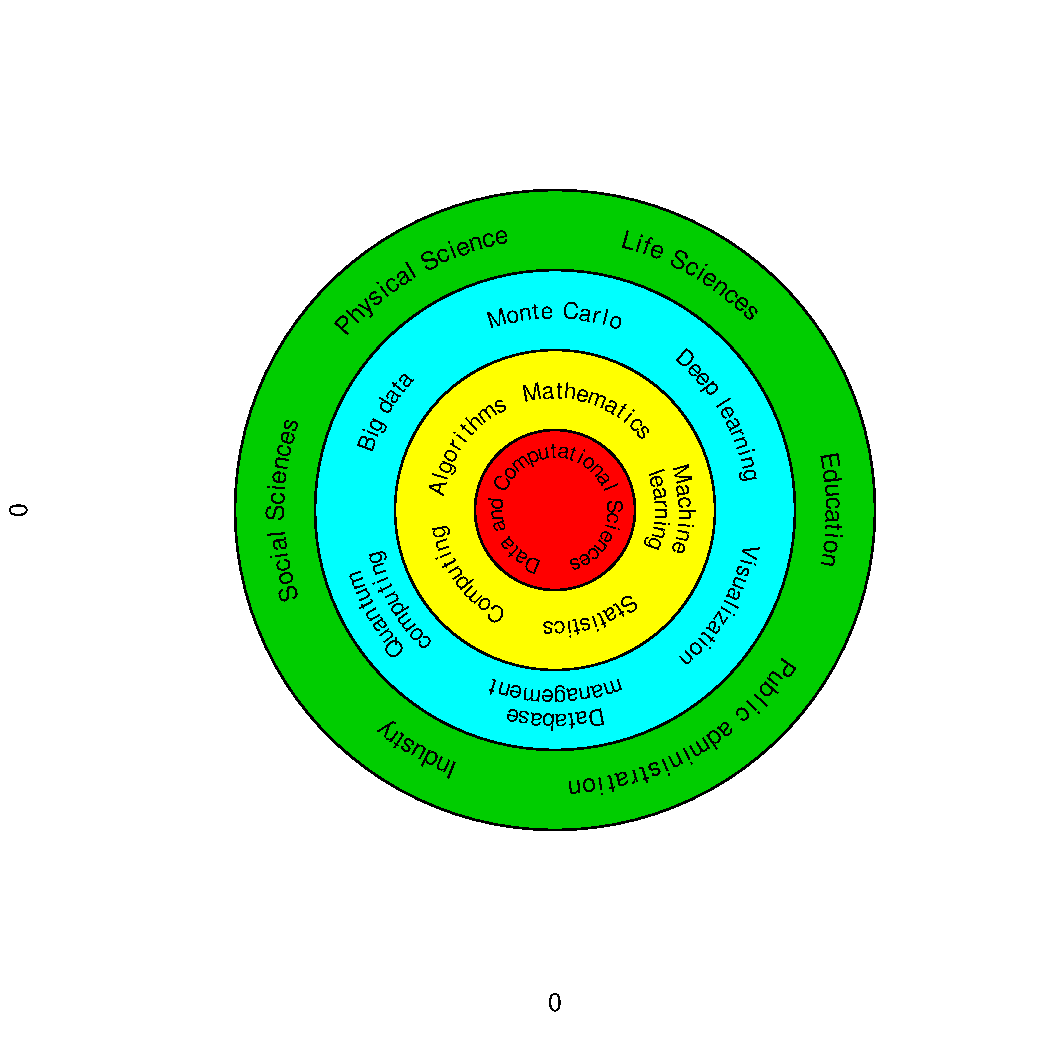
\includegraphics[width=0.5\textwidth,trim={3.7cm 2.9cm 1.6cm 2.4cm},clip]{DASCO.pdf}
\caption{\label{fig:dept}Major discipline (yellow), some suggested topics (cyan), domain areas (green).}
\vspace*{-1cm}
\end{wrapfigure}

At the research level, the center should not aim at covering all
topics within DS and CS but rather select some areas where we have
high chances of succeeding. The selection of such topics will depend on which
researchers that choose to be part of the center. Some possible
subjects are listed below.

\cleapage



\paragraph{Deep learning} has revolutionized image analysis (using convolutional and recurrent networks) with considerable success in  many other areas of applications as well. Network structure and Bayesian model selection are active research areas at both IFI and MI.
\todo{ AS: Today, deep networks can appear like a black box, and research will be focused on understanding  the mechanisms behind the decisions that the network makes, e.g. in terms of reliability, robustness, and the associated uncertainty.  This is an area where the joint competence of the center really can make an impact to merging applications in e.g. machine vision, robotics, and language models tighter with traditional statistical modelling. 
Another interesting area is learning for imbalanced data set, which is typically for many applications in e.g. medicine. Models for incorporating prior knowledge into deep networks is also an area where the joint cross-disciplinary comptence will create large potential. 
The link to optimization is also very strong, and the potential for developing better learning algorithms is large. }



\paragraph{Big data} The volume of data continues to increase exponentially. The amount of data poses challenges both in construction of concepts on how to analyze such data computationally.
In many cases, the data are of the observational type, in that data comes first, what to do with the data second. In such cases one needs to consider whether the data are relevant for the purpose of the problem. Also traditional statistical approaches  needs to be reconsidered in big data settings (such as the use of false discovery rates instead of more traditional correction for multiple testing).
High-dimensional data occur frequently but is typically related to sparsity in the parameters or subspaces that explain insight. Traditional methods typically have problems in such cases and new methodology is needed. Computational challenges frequently occur in big data settings and development of scalable algorithms is an active research field today. 

\paragraph{Reinforcement learning}

\paragraph{Privacy}

\paragraph{Transparency/reproducibility}


\paragraph{Data Access}

Before data can be analysed (be it using statistical methods, finite elements, etc.) it must be made available in a suitable format, and with sufficient data quality.  In industrial applications this often involves gathering data from a number of different data sources, spread over the enterprise, and massaging it to overcome differing data models and encodings.  This task of Data Access often takes more time than the actual analysis.  Formal management of available data sources and their semantics can automate these tedious and error prone processes.

It is beneficial to see data access and analysis as interacting parts of a data science pipeline: the same formal domain models that are used for data integration can be used to make statistical analysis more domain-aware; and statistical methods can be used to uncover data quality problems that can be addressed as part of data access.

\paragraph{Hybrid Inference}

Many industrial applications of machine learning methods are characterized by a) a comparatively limited amount of data, but b) large amounts of structured information in databases, business rules, formal domain models, etc.  Domain knowledge is usually included in the data science pipeline in \emph{ad hoc} ways, through the understanding of data wranglers and data scientists.  A more principled approach to the combination of \emph{logical inference} (i.e.~processing of hard facts) and \emph{statistical inference} will systematically lead to more useful conclusions and predictions, that are consistent with available domain knowledge.


\paragraph{Monte Carlo methods} or stochastic simulation is an important computational tool within both Data Science and Computational Science. It is highly used in physics and astrophysics as well as in many Bayesian approaches within statistics and the faculty has several methodological researchers within this field. Traditional Markov chain Monte Carlo methods are typically very slow and modifications/fine tuning are often necessary for use in modern research problems. Subsampling, divide-and-conquer approaches, use of auxiliary variables 
are some examples of methods that have been proposed. There are also alternative strategies such as sequential Monte Carlo and approximate methods (variational inference).

\paragraph{Optimization}
\todo{AS: We could add something along the lines that today in deep learning, very naive first order methods are used. Most commom is perhaps stochastic gradient descent with momentum, decaying learning rate, or simple methods for adaptive updates of the different weights like Adam. A large potential is probably also to use Bayesian grid searches for the hyperparameters.}

\paragraph{Quantum computing} \todo{This part needs to be shortened somewhat}Enabling simulations of large-scale quantal many-particle systems is a long-standing problem in scientific computing. Quantum many-particle interactions define the structure of the universe, from nucleons and nuclei, to atoms, molecules, and even stars. Since the discovery of quantum mechanics, a lot of progress has been made in understanding the dynamics of certain many-particle systems. While some of our insights come from a small set of analytically solvable models, numerical simulations have become a mainstay in our understanding of many-particle dynamics. The progress in numerical simulations has accelerated in the last few decades with the advent of modern high performance computing (HPC) and clever developments in classical simulation algorithms such as, quantum Monte Carlo,large-scale diagonalization approaches, and other renormalization schemes. Despite the monumental advances, classical simulation techniques are reaching fundamental limits in terms of the size of the quantum systems that can be processed. Fortunately, the disruptive new field of quantum simulations has emerged, promising to enable simulations far beyond those which are classically tractable. 

Recent progress in quantum computing as well as digital and analog Quantum Algorithms (QAs) promise to enable the exciting possibility of performing simulations that are beyond the reach of all existing and future classical supercomputers. Despite the progress, there is still a gap between the resources required by state-of-the-art QA and the resources offered by available and near-future quantum hardware. It may take decades of quantum hardware development and engineering before the current QAs will outperform classical exascale class simulations. Therefore, to impact scientific computing on a more relevant time scale, improving the scalability and efficiency of quantum simulation algorithms is of the highest importance. Developments in quantum information algorithms and their mathematical properties, as well as their applications will play a critical role in studies of relevance for a wide variety of fields, from the design and studies of new materials to our basic understanding of systems of interest in chemistry and physics. The new center, in close collaboration with disciplinary experts, can play an essential role in developing this field by hiring world-leading experts in quantum information theory and quantum computing.

\paragraph{Visualization}


\subsection{Challenges}
Creating such a center will pose some challenges. We have listed some below that should be considered. 
\begin{itemize}
\item Time-frame: New related centers and education programs appear at several other universities. We need to move quickly in order to not be left behind, both in attracting students and on outside collaborators. The center should be established within the first half of 2020.
\item Location: It is important that a co-location is established at the start of the center-period in order to kick off collaborations as soon as possible. 

\item Relations to other centers: OCBE, NR, Simula, Sintef, Nora-centers, Startup-Lab. These are all environments that also operate in the CS/DS area. How to formally or informally collaborate with these centers should be considered.
\item Relations to other CS/DS studies. Several other programs at the MN faculty include flavours of CS/DS topics. The current master programs in DS and CS have different approaches to this. CS includes many domain-specific directions while DS has a more pure methodological profile combined with offering more user-friendly courses that can be included in the domain-specific programs.   
\item Organization at the Department for Informatics 
\end{itemize}
 Regarding the last point: Today, research in machine learning is distributed to research sections for Bioinformatics,   Digital Signal Processing and Image Analysis, Language Technology, and Robotics and intelligent systems. A reorganization to increase cooperation and visibility  is likely to happen at IFI. A likely scenario is a section for Machine Learning, either as a new section at the same level as existing sections, or a reorganization of the entire section structure, to add a section level on top of today's structure. This proposal can be seen as a scenario where selected staff at IFI have a joint position at the DASCO-center. IFI will also strengthen the theoretical competence in ML through future positions, but they will still be tailored to solving theoretical problems related to applications in biomedicine, imaging, language, or robotics. Deep learning through convolutional networks,  recurrent networks, or reinforcement learning are the driving forces for ML-activities at IFI.  




\appendix
\section{Appendix}
\subsection{Mandat}\label{ap:mandat}

Data Science (DS), inkl. maskinlæring, og Computational Science (CS) er svært viktige
områder ved Det matematisk-naturvitenskapelige fakultet. Det ble for eksempel startet
nye masterprogrammer på disse to områdene høsten 2018. Begge programmene har mange
søkere, det er stor interesse for enkeltemner innen DS og CS, og sist men ikke minst er
kandidatene med kompetanse inne DS og CS svært ettertraktet i arbeidsmarkedet.

Fakultetet har gjennom det siste året jobbet med ny strategi som peker mot hva
fakultetet vil være og oppnå fram mot 2030. I løpet av høsten skal dette strategiarbeidet
gå over i utviklingen av en handlingsplan for perioden 2019-2021. Hva fakultetet skal satse
på innen DS+CS og hvordan fakultetet best kan organisere og støtte opp om denne
aktiviteten er ett av flere viktige spørsmål som må besvares i en slik handlingsplan.
Fakultetet nedsetter derfor en arbeidsgruppe som skal komme med anbefalinger om
satsingen innen DS+CS ved fakultetet. Arbeidsgruppen skal som utgangspunkt fokusere
på den delen av denne virksomheten som er forankret i matematiske fag, herunder
statistikk og beregninger.

I et lengre perspektiv er det ventet at en satsing på DS+CS vil påvirke hele fakultetet (og
andre deler av Universitet i Oslo). Arbeidsgruppen skal derfor rapportere til dekanat
underveis i arbeidet og en underveisrapport skal legges frem for instituttledermøtet.

I dette arbeidet vil det være spesielt viktig å skissere arbeidsgruppens anbefalinger og
hvordan forholdet er og bør være til fakultets øvrige aktiviteter innen DS+CS, dvs. de deler
som ikke faller innen under den fokusering som er uthevet over. Dette vil typisk være
aktiviteter som benytter maskinlærings-teknikker i studier av vitenskapelige eller anvendte
problemstillinger og viktige deler av DS+CS (særlig DS) som har sin vitenskapelige
forankring i informatikk, for eksempel kunnskapsrepresentasjon (digital representasjon) og
kunstig intelligens.

Presiseringer i mandatet
\begin{enumerate}
\item Gi en kort statusoversikt over forskning og undervisning/utdanning innen DS og CS
ved fakultetet med den avgrensning som er skissert over.
\item Utdanning: Peke på utfordringer for våre nye studieprogrammer innen DS og CS
(f.eks. rekruttering av studenter, ressurser, veiledersituasjon, kapasitet, behov
framover for slike kandidater).
\item Forskning: Peke på utfordringer knyttet til det å skape fruktbart, tverrfaglig
samarbeid på fakultetet der DS og CS inngår, herunder beskrive hvordan DS og CS
bør styrkes for å oppnå en ønsket situasjon.
\item Drøfte samfunnsdelen av DS+CS, herunder kontaktflater og samarbeid med
næringsliv/ forvaltning og resten av UiO.
\setcounter{save}{\value{enumi}}
\end{enumerate}
Arbeidsgruppen skal levere en underveisrapport på punktene 1-4 innen utgangen av 2018.
Denne rapporten skal være grunnlaget for en diskusjon i dekanat/instituttledermøtet
(tidlig januar 2019). Basert på denne diskusjonen bes arbeidsgruppen om å ferdigstille sin
rapport, som også skal adressere punktene 5-6, innen 1. februar 2019.
\begin{enumerate}
\setcounter{enumi}{\value{save}}
\item Sette opp naturlige strategiske ambisjoner/mål for fakultetet innen DS+CS.
\item Foreslå tiltak for å nå disse målene, for eksempel organisering, aktiviteter,
ressursbehov, finansiering av nye stillinger, profilering, samarbeid etc.
\end{enumerate}
Det forutsettes at arbeidsgruppen involverer aktuelle miljøer som ikke er representert i
arbeidsgruppen.

Den ferdigstilte rapporten skal behandles i dekanat/instituttledermøte.

\subsection{What is Data Science and Computational Science?}

\subsubsection*{What is Data Science (DS)}
Data science (DS) has grown into a separate scientific field, both due to the exponential growth of available data and due to the emerge of new methods and algorithms to analyse these, but perhaps the most important part is the potential value that companies sees in data-driven decision making. 
There are various definitions of DS, but the most common definitions describes DS as the whole process of discovery, knowledge extraction and decision making based on data. It includes definition of questions of interest, data collection and preparation, exploratory analysis, modelling, evaluation and presentation of results.  
Data science blends statistical and computational thinking. The art of data science is to understand how to apply the tools available in the context of a specific dataset and for answering specific (scientific) questions, but also deciding which data to acquire, making the human perspective even more important than before (in contrary to the belief that modern machine learning tools can be used as black boxes).
Donoho (2017) defines DS as the union of six areas:
Data gathering, preparation, and exploration.
Data representation and transformation.
Computing with data.
Data modeling.
Data visualization and presentation.
Science about data science.
Statistics and computer science are core … with mathematics as an important basis. In short one can say that Data Science is the science of extracting knowledge or insight from various types of data. 

Carmichael and Marron (2018): Data science is the business of learning from data, which is traditionally the business of statistics. Data science, however, is often understood as a broader, task-driven and computationally-oriented version of statistics.

Machine learning techniques are in many cases presented as the main tools within Data science, but many other tools and fields such as database management, web-scrapping, visualization etc are equally important. 

Applications of Data Science tools are today spread around the whole faculty, and also at other faculties (medical, social science). However, methodological development within Data Science is mainly concentrated around Department of Mathematics (section 2) and Department of Informatics (sections …) with smaller research groups perhaps also at Department of Physics and ?? In addition, the research group in biostatistics at the medical faculty does methodological work in data science.

A main problem within machine learning today is the hype that such tools can be used as black boxes and solve any kind of problem. It is important to recognize that the computer is just a tool to perform the computing necessary while the main challenge is to decide what to compute!
Further, the explosion of data in many cases requires more modelling, not less. An example is the “p larger than n” settings occurring for example in genomics. With few individuals, extracting information makes it necessary to constrain models rather than expanding them.
The data growth also include non-standard and complex data, also requiring more modelling than less






 
\subsubsection*{What is Computational Science (CS)}
Computational science refers to the use of computers, networks, storage devices, software, and algorithms to solve problems, do simulations, build things, or create new knowledge. Computational Science can be viewed as the intersection of: 
Computing and networking hardware
Algorithms, Numerical Analysis, and Mathematics
Software, Programming, and Databases
Discipline specific knowledge

It is an incredibly broad discipline. The Institute of Electrical and Electronics Engineers (IEEE) states: 

The term Computational Science presents a broader view, implying science (and engineering) that is "computational" as opposed to "experimental" or "theoretical" in nature. Computer Science, of course, deals with the science and engineering of computers. 
Some areas of computational science require large computers to perform trillions of floating point operations (computational fluid dynamics, computational chemistry, computational meteorology, computational physics, etc.). Other areas of computational science build and utilize large databases and require terabytes of storage (bioinformatics, business, knowledge management, geographical information systems, etc.). And some areas will require networks of computers to accomplish their goals (web technologies, grid computing, collaborative software, systems of systems, online communities, etc.). Graphics and visualization are also important areas. The most exciting computational science problems might involve all of these: computing, data storage, and networking (e.g. artificial intelligence, computational steering, mobile robots, virtual reality, etc.). Software development and programming are also crucial parts of computational science (e.g. Java, C++, MPI, CORBA, OpenGL, mySQL, PHP, Perl, Linux, etc.). 

Computation is now regarded as an equal and indispensable partner, along with theory and experiment, in the advance of scientific knowledge and engineering practice. Numerical simulation enables the study of complex systems and natural phenomena that would be too expensive or dangerous, or even impossible, to study by direct experimentation. The quest for ever higher levels of detail and realism in such simulations requires enormous computational capacity, and has provided the impetus for dramatic breakthroughs in computer algorithms and architectures. Due to these advances, computational scientists and engineers can now solve large-scale problems that were once thought intractable. Computational science is often thought of as the third leg of science along with experimental and theoretical science. 
 
 
 
 





\subsection{Results from survey}
\begin{wrapfigure}{r}{0.3\textwidth}
\centering
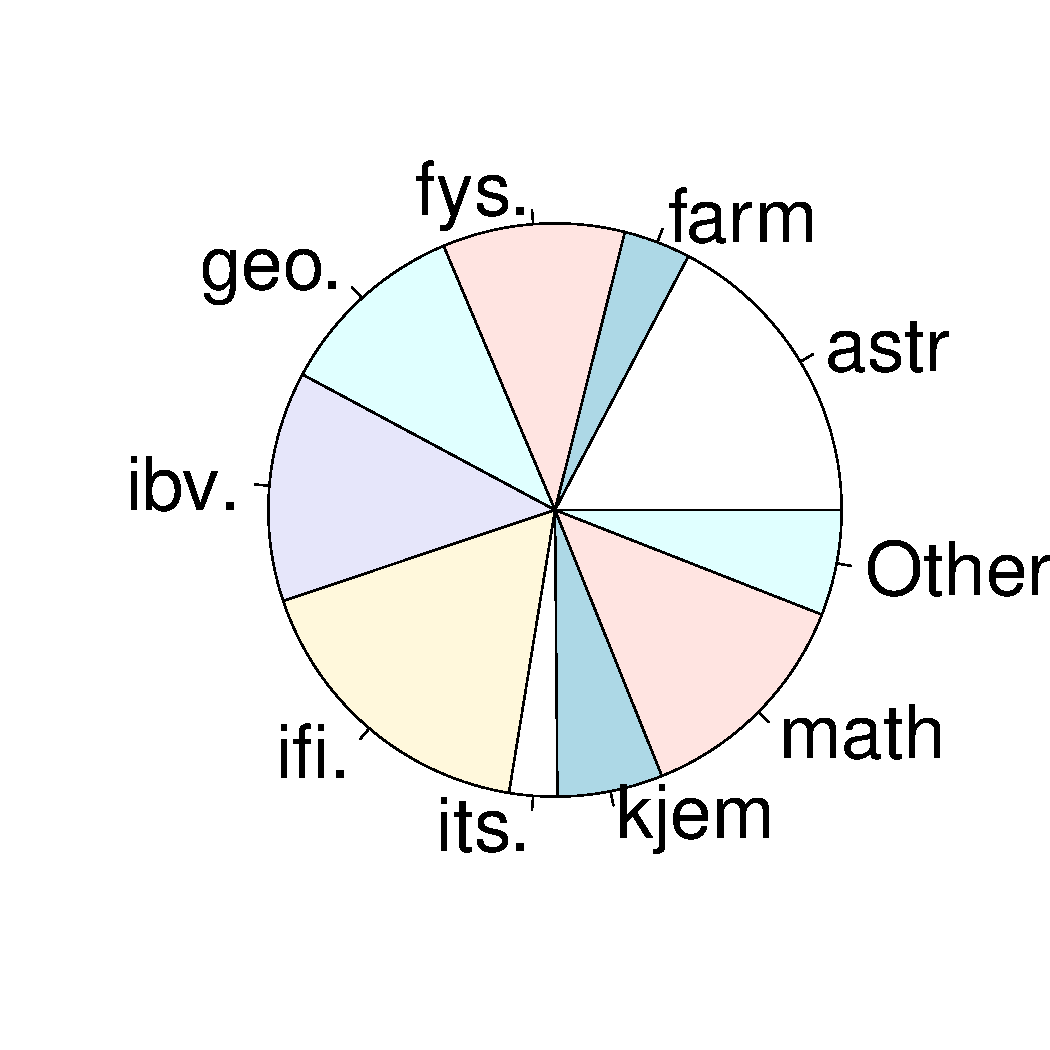
\includegraphics[scale=0.3,trim={0.5cm 2.7cm 0cm 2.4cm},clip]{pie_dept.pdf}
\caption{\label{fig:deptdistr}}
\end{wrapfigure}
A survey on activities within the MN faculty was performed fall 2018. A total of 185 participated in the survey with most interest at Astro, Physics, GeoScience, Ifi and Math.
Others include Simula, Sintef, SV-fak, MED-fak and some students, see Figure~\ref{fig:deptdistr}. As expected, mainly those at least somewhat interested in either Data Science or Computational science did respond on the survey. However, there is probably a large number of researchers that are interested in these fields, that did not respond to the survey. The survey do however give some indication of the interest in DS/CS as well as how the fields are distributed over the departments within MN. 


\paragraph{Question} \textit{How important is DS/CS in your research?}\\

\begin{center}
\begin{tabular}{rrrr}
\multicolumn{4}{c}{Table of importance of DS vs CS}\\
  \hline
 DS$\backslash$ CS& Not important & Somewhat important & Very important \\ 
  \hline
Not important &  10 &   3 &   8 \\ 
  Somewhat important &   4 &  13 &  35 \\ 
  Very important &   7 &  22 &  82 \\ 
   \hline
\end{tabular}
\end{center}

\begin{center}
\begin{tabular}{rrrrrrr}
\hline
\multicolumn{7}{c}{Importance distributed over units, first DS and then CS}\\
  \hline
 &\multicolumn{2}{c}{Not important} &\multicolumn{2}{c}{Somewhat important}&\multicolumn{2}{c}{Very important} \\
 &DS&CS&DS&CS&DS&CS\\
  \hline
astr &   2 &   0 &   7 &   1 &  23 &  31 \\ 
  farm &   1 &   1 &   3 &   4 &   3 &   2 \\ 
  fys. &   3 &   1 &   5 &   2 &  11 &  15 \\ 
  geo. &   0 &   0 &   8 &   2 &  12 &  18 \\ 
  ibv. &   1 &   2 &  10 &   9 &  13 &  13 \\ 
  ifi. &   4 &   8 &   5 &   7 &  23 &  17 \\ 
  its. &   0 &   1 &   2 &   0 &   3 &   4 \\ 
  kjem &   3 &   1 &   4 &   3 &   4 &   7 \\ 
  math &   7 &   6 &   6 &   7 &  11 &  11 \\ 
  Others &   0 &   1 &   2 &   3 &   9 &   7 \\ 
   \hline
\end{tabular}
\end{center}

A large percent answered that both topics are very important, indicating that there is a large overlap in use of these methods. In addition to the two methodological oriented departments (MI and IFI), several other departments have many researchers that find these fields to be very important.

\paragraph{Question} \textit{If Data Science/Computational science plays a role in your work, how are you involved?}\\

\begin{tabular}{rrrrrrrrrrr}
  \hline
  
 & astr & farm & fys. & geo. & ibv. & ifi. & its. & kjem & math & Others \\ 
  \hline
Apply DS/CS to new probl &  21 &   5 &  10 &  14 &  19 &  14 &   5 &   6 &   2 &   5 \\ 
  New method. in CS &   8 &   0 &   3 &   3 &   0 &   6 &   0 &   2 &   8 &   2 \\ 
  New method. in DS &   3 &   0 &   2 &   3 &   2 &   9 &   0 &   2 &  10 &   3 \\ 
   \hline
\end{tabular}\\

At most departments, applying DS/CS methodology is the main focus. Developing methodology has more focus on IFI and MI, but also at Astro!

\paragraph{Question} Is it natural/interesting for you to supervise Master students in the new Data Science program?

\begin{tabular}{rrrrrrrrrrrr}
  \hline
 && astr & farm & fys. & geo. & ibv. & ifi. & its. & kjem & math & Others \\ 
  \hline
No&DS &   9 &   3 &   9 &   5 &   7 &   7 &   2 &   6 &   9 &   3 \\ 
  &CS &   6 &   3 &   5 &   2 &   9 &  13 &   2 &   3 &   8 &   4 \\ 
To some extent&DS &  14 &   4 &   7 &   9 &   9 &  14 &   0 &   4 &  11 &   3 \\ 
              &CS &  14 &   4 &   9 &  11 &   9 &  12 &   0 &   7 &  11 &   4 \\ 
  Very &DS&   9 &   0 &   2 &   5 &   7 &  11 &   3 &   1 &   4 &   5 \\ 
       &CS&  12 &   0 &   4 &   7 &   6 &   7 &   3 &   1 &   5 &   3 \\ 
   \hline
\end{tabular}

\paragraph{Question} \textit{Do you think Data Science and/or Computational Science will play an increasing role in your future research? If so, please write a couple of sentences on this.}

Most respondents answer that DS or CS will be important in their future research
Among 143 responses, 56 mention computing in their responses, 94 mention data while 38 mention both DS and CS.
Themes that are mentioned are astrophysics, bioinformatics, biology/medicine, buisiness, chemistry, climate, cyber security, 
database management, ecology, energy,  genomics, imaging, geoscience, material science, natural language, robotics,
physics and teaching showing that DS and CS are applied
in a wide range of topics. 
Several mention that DS and CS give the possibility to work with more realistic models.


\subsection{Education in DS and CS at MN/UiO}

Education in DS and CS at MN/UiO can be divided into specific programs which specialize in Data Science and courses which cover different topics within Data Science and Computational science. 


Programs and courses
\begin{itemize}
\item Two new (from fall 2018) Master of Science programs in Data Science and Computational Science tailored to STEM fields. These are specialized programs aiming at educating methodologically strong candidates.
\item An option in Statistics and Data Science within the MAMI bachelor program. There are also other bachelor programs that have a solid mathematical basis (MAT1100/1110/1120) that potentially can lead to further studies in Data Science or Computational Science (e.g physics, astronomy, geophysics). 
Several other  bachelor programs and/or study options can also qualify for the above mentioned master programs.
\item A wide range of courses in DS and CS, mostly within MI and IFI but also at other departments, see Tables~\ref{tab:DScourses} and~\ref{tab:CScourses}.
There is a lack of coordination of these courses.
\item An increasing number of master students within other scientific fields are using DS and CS, in particular machine learning algorithms. Supervision of such students are in some cases problematic since many of the supervisors lack research competences and skills in machine learning. In particular there has been a demand for statisticians to aid with for example co-supervision of students. Unfortunately, the number of faculty with such skills and competences is strongly limited at the Faculty of Mathematics and Natural Sciences.
\end{itemize}
\begin{table}[t]
    \centering
    \tiny
    \begin{tabular}{llll}
    \hline
STK2100 & Machine learning and statistical methods&
STK-INF3000/4000 & Selected Topics in Data Science\\
&for prediction and classification&STK4021 &Applied Bayesian Analysis\\
STK4051 & Computational statistics&
STK-IN4300 & Statistical learning methods in Data Science\\
IN3050 & Introduction to Artificial&
IN4080 & Natural Language Processing\\
& Intelligence and Machine Learning&INF4490 & Biologically Inspired Computing\\
IN-STK5000 & Adaptive Methods for Data-Based Decision Making&
IN5400 & Machine learning for image analysis\\
TEK5040 & Deep learning for autonome systems&
TEK5020 & Pattern recognition\\
FYS-STK3155/4155 & Applied data analysis and machine learning&
GEO4310 &Stochastic methods in hydrology\\
\hline
\end{tabular}
\caption{Courses that have a large component of Data Science topics included}
\label{tab:DScourses}
\end{table}

\begin{table}[t]
    \centering
    \tiny
    \begin{tabular}{llll}
    \hline
MAT3360& Introduction to PDE&
MAT4110& Introduction to Numerical analysis\\
MAT4120& Mathematical Optimization&
MAT4130& Numerical Analysis\\
MAT4160& Topics in Geometric Modelling&
MAT4301& PDE\\
MAT4305& PDE and Sobolev spaces I&
MAT4315& PDE and Sobolev spaces II\\
MEK4250& Finite Element Methods &
MEK4470& Computational Fluid Mechanics\\
FYS3150/4150& Computational Physics I\\
FYS4411& Computational Physics II&
FYS4460& Computational Physics III\\
INF4300& Digital image analysis&
INF4331& Problem solving with high level languages\\
INF5620& Numerical Methods for PDE&
INF5631& Project on Numerical Methods for PDE\\
INF5670& Numerical methods&
INF5840& Computability theory\\
& for Navier-Stokes equations&INF5560& Computational Physiology\\
GEO4300& Geophysical Data Science\\
GEO4510& Digital Terrain Aanalysis&
GEO4900& Atmosphere Ocean Dynamics\\
AST5210& Stellar Atmospheres I&
AST9110& Numerical Modeling\\
INF4350& Introductory Course in Bioinformatics&
INF-BIO5121& High Throughput Sequencing technologies\\
INF5380& High-performance computing in bioinformatics&
& and bioinformatics analysis\\
MBV3070& Bioinformatics&
MBV-INF4410& Bioinformatics for Molecular Biology\\
STV1515& Programmering og maskinlæring for samfunnsvitere\\
SOS290& Algoritmer, store data og samfunnsendring\\

 \hline
\end{tabular}
\caption{Courses that have a large component of Computational Science topics included. Partial differential equations abbreviated as PDE.}
\label{tab:CScourses}
\end{table}

\newpage
\subsection{Research in DS and CS at the Faculty of Mathematics and Natural Sciences}
This section describes research activities within DS and CS at the Faculty of Mathematics and Natural Sciences. This description is most likely not complete. We apologize for eventual shortcomings and urge the attentive reader to aid us in improving the quality of this document. 
\subsubsection*{Department of Mathematics}
Most of the research within DS at MI is concentrated around the analytics part of the Data Science workflow. This both involves development of new sophisticated data-driven “machine learning” tools and making more traditional model based tools useful for big data settings. It involves extending/modifying models to new settings, deriving more efficient algorithms and deriving mathematical properties of the methods involved. It also involves applying machine learning tools to new applications. Much of the development of new methods is performed at section 2 (Statistics and Data Science), but several other sections have some activity or interest in the area of machine learning. The people at section 2 involved in this area are  Ørnulf Borgan, Riccardo De Bin, Ingrid Glad, Ingrid Hobæk Haff, Geir Storvik, Ida Scheel, and some adjunct professors. 
Most of the research within Data Science is performed through PhD projects, many which are sponsored by the SFI BigInsight. 

Through the SFI BigInsight, but also through other projects, there is an extensive collaboration with industry and public administration (DNV-GL, ABB, DNB, Gjensidige, Telenor, Hydro, OUS, SSB, Skatteetaten, NAV, Folkehelsa, PRIO, NR +++).
There has also been an increasing interest in the “Nærings-PhD” options with many inquiries from external companies having specific projects and candidates ready. Due to capacity problems, many of these requests have been turned down (but we have næringsphd with DNV-GL, ABB, Finn, +1)
We also see an increasing number of requests to participate in projects from other fields were Data Science/machine learning methodology is required (Prio, IBV, Rettsvitenskap, ...) 

At MI there is activity related to CS in several sections, in particular in the groups in mechanics, partial differential equations, reliability/risk analysis and geometrical modeling. 


\subsubsection*{Department of Informatics}
	 	 	 	
At IFI, the research in DS is strongly linked to application areas in the sections Biomedical Informatics (BMI) , Digital Signal Processing and Image Analysis (DSB), Language Technology (LTG), and Robotics and Intelligent Systems (ROBIN). These sections have a long tradition for applying statistical methods in research problems in deriving information from applications in speech (LTG), images (DSB), and robotics (ROBIN)… BMI.

Recent advances in machine learning has impacted almost all the sections at IFI to include activities in machine learning, but for BMI, DSB, LTG and ROBIN a central part of the research is based on machine learning. The focus is mostly on applications, and to extract information from data.
With the success of deep learning particularly in robotics, speech technology, and image analysis, we currently see a shift in methodology in the direction deep learning using convolutional and recurrent networks, but traditional machine learning methods for feature extraction and classification are also studied.
The SFI SIRIUS focuses on the data handling/Big data part of DS, not the machine learning part.

All of the sections have in increasing demand from external companies to participate in cooperative projects, but the capacity is limited. There is a also a high need for competence in supervision students on machine learning problems.

In terms of CS at IFI, several of the sections do research where heavy computations/large simulations/large datasets are in focus. The methods are applied for applications, e.g. signal processing or biomedical computing. Access to a range of facilities for computation, ranging from desktop computers with GPU, servers with GPU, the Condor system for distributed computing, and large computing facilities like Abel.




\subsubsection*{Department of  Geosciences}
Geoscience has long been a computationally-intensive area. A typical climate simulation, used for example in the future projections discussed by the Intergovernmental Panel on Climate Change (IPCC), can generate a petabyte (1 million gigabytes) of data. Weather forecasts involve suites of complex simulations, which are then averaged to assess the probability of different scenarios. These models simulate not only the atmosphere, but the important interactions with the ocean, land and vegetation. Sophisticated models are also used for studying tectonic continental shifts, to understand the geology and climate of previous epochs, thereby informing our understanding of prehistoric life. And similar models are used to simulate hydrological reservoirs and the melting occurring at the base of major glaciers. Computation is so central to the geosciences that it is impossible to imagine the study without it.
The computational approaches relevant for geoscience can be grouped in two classes: simulation and analysis. Geoscientific computation demands advanced programming techniques and optimized simulations, to ensure the fast calculations. Changes in the global ocean circulation can take tens of thousands of years, demanding the most rapid simulations possible. High performance computing approaches, for example using graphical processing units (GPUs), are now being applied to climate models, greatly increasing performance. The large amount of data generated by geophysical simulations is also a challenge and is well-suited for big data techniques. Machine learning is beginning to be used in weather forecasting and in climate simulations. This has led to the identification of weather patterns missed by researchers and to the identification of extreme events like cyclones and “atmospheric rivers”, on par with that of human analysts. Computational geoscience is an exciting and developing field, and one which will make major inroads to the earth sciences in the future.

\subsubsection*{Department of Biosciences}
Life Science is being transformed with the explosion of high-throughput data generation technologies and the need for integrating these across all the levels of the biological hierarchy. A 'system-dynamic' (Systems Biology) approach will dominate research in the coming decades. Here, data analytics tools for handling big data and computational modelling to integrate the various data types and data sets will be a driving force. Similar developments are seen in the field of molecular image analysis, where computational methods to integrate the image streams will become essential to make sense of the growing amount of data. Translational Bioinformatics, bridging the gap between the laboratory, computer and the clinic, with the ultimate goal of personalised medicine, is an important, and exciting new dimension. Many of these developments require cross-disciplinary thinking, and often breakthroughs in Bioinformatics/Computational Life Science start with creatively adjusting and implementing algorithmic or computational solutions originally developed for other fields.  The department of Bioscience has also a strong activity in computational neuroscience linked to the experimental programs. This entails solutions of differential equations, handling of large data sets and machine learning. In addition, the department has a long history in (sophisticated) statistical analysis of more traditional ecological data.

\subsubsection*{Department of Chemistry}

The Hylleraas center of excellence in computational and theoretical chemistry is a typical example of where a large variety of algorithms for solving quantal many-body problems play a central role. These algorithms span the whole spectrum of central methods in computational science, from large eigenvalue problems to stochastic simulations, large systems of non-linear equations and systems of ordinary and partial differential equations. High-performance computing with CPU and GPUs play a central role and the applications span from material science to a fundamental understanding of reactions. Many of the research groups are involved with multi-scale problems, where an understanding of methods that apply to a certain length and energy scale and how to link different scales plays a central role. Machine learning is being used in the analysis of theoretical and experimental data.
\subsubsection*{Research in DS and CS at the Institute for Theoretical Astrophysics}
The Institute of Theoretical Astrophysics is one of the strongholds at the university of Oslo when it comes to applied DS and CS, spanning from large scale data analysis from the Planck satellite to massive high-performance computing of the physics of the sun. The latter involves solutions of complicated sets of coupled partial differential equations whereas the cosmology activity includes  the development and applications of a large variety of numerical algorithms, from   Monte Carlo simulations, Machine Learning, statistical data analysis to optimization problems. The institute, together with the department of Chemistry host some of the more successful centers of excellence in Data Science and Computational Science in Norway. A large swath of algorithms from DS and CS are studied and developed in order to study phenomena of astrophysical interest. 
\subsubsection*{DS and CS in Education Research (Center for Computing in Science Education)}


Quantitative education research has historically been done at the micro-scale (classrooms) and the macro-scale (K-12, baccalaureate degree programs, etc.). Micro-scale research has been done using traditional correlational statistics with data gathered from surveys, conceptual tests, classroom observations, etc. With the advent of the digital classroom, student behavior can now be examined in fine grain. Students access of online homework platforms, video lectures, and interactions with peers via online course forums has created new data sources for education researchers. New technologies such as computer textual analysis can pick apart student conceptual understanding of hard concepts in science and mathematics. Intelligent tutors can provide real time feedback to students as they solve problems. At the macro-scale students’ career decisions within their programs can be modeled. What courses they choose to take, who they choose to take courses from, and their comments on said courses, form new data sets which can be used to predict student decisions and provide timely feedback to students and faculty advisers. Ultimately these data sets can form a high dimensional picture of student learning painted by machine learning.

\subsubsection*{Department of Physics}

The department of Physics has Computational Science and Data Science activities in several of its research groups. Some of the research groups use mainly existing software in the their analysis of for example experimental data. This is particularly relevant for the experimental research activities in subatomic physics (high-energy physics and nuclear physics). In high-energy physics there is a long tradition in using machine learning in the analysis of experimental data. Experimenters at CERN started using Machine Learning algorithms more than twenty years ago. The huge amount of data from experiments at CERN requires that the  high-energy physics group is heavily involved in both development and usage of CS and DS software. Furthermore, there is strong need for large storage capacities and high-performance computing resources (software and hardware).  
The applications and developments of DS and CS algorithms and software is also important to activities in space physics, condensed matter physics and biophysics. In particular, Monte Carlo methods and  the solution of ordinary and partial differential equations play a central role. 
The Department of Physics has also a group in Computational Physics. The group has worked with computational methods tailored to studies of strongly interacting quantum mechanical systems, spanning from atoms and molecules to condensed matter and materials science to subatomic physics. The latter includes Lattice quantum chromodynamics and studies of nuclear matter. The methods range from stochastic simulations (Monte Carlo methods) to solutions of large eigenvalue problems and large sets on non-linear equations. Optimization problems are used extensively. A broad spectrum of algorithms in computational science are used and developed, in addition to statistical data analysis and Machine Learning algorithms. The main activities have focused on computational quantum mechanics and computational statistical mechanics. The group collaborates with researchers across the disciplines, from political science to meteorology, mechanics and computational neuroscience.  Many of the above methods are widely used by other research groups at the department of Physics. Compared with the Departments of Chemistry, Geosciences and Theoretical Astrophysics, CS and DS research at the department of Physics has used less of the national high-performance computing resources.\todo{HS: Jeg er ikke sikker på om dette stemmer, eller vi bør legge til en kommentar at det er fordi vi har stor bruk av  internasjonale ressurser} This is likely to change in the future.

The Computational Physics group has also been central in the development of the Computing in Science Education project, a project which aims at integrating in a coherent way computing in basic science courses. The members of the group are central members of the newly established Center of Excellence Center for Computing in Science Education. 
The group has also developed several highly popular courses in computational physics, amongst these FYS3150/4150 with approximately 100 students from all disciplines in natural science at UiO. The members of the group have also developed the new course on Data Analysis and Machine Learning, FYS-STK3155/4155, with close to 100 students when it run the first time during the fall semester 2018. The members of the group initiated the process that led to the establishment of the new Master of Science program Computational Science. 



\subsubsection*{DS and CS Research in other Fields}

A strong emphasis on DS and CS has the potential to develop novel collaborations across disciplines. Data analytics has a long history within Social sciences (in particular economics). In the Humanities and the Social Sciences there are several examples where Machine Learning starts to play a central role. Strengthening research in DS and CS with Machine Learning are research areas of great interest where the departments of Mathematics and Informatics can play a central role in establishing new research and educational activities. We list here some possible examples:


\paragraph{Computational Psychology}
Large files of audio/video are currently unused since data is in a form that is unavailable for quantitative analysis (such as video of weekly clinical interviews from multi-center trials of treatment for thousands of patients). Analysis of prosody can shed light on change processes, and should automatic transcription reach a sufficiently good level, this will, in combination with natural language processing, open up many interesting research questions.
Accumulated data from online use already provides measurements of quantities such as personality, attitudes, skills or mental disorders which in many cases have proven to approach the level of the best instruments we have. Here one obtain much more, especially since clinical treatment will increasingly be supplemented by electronic registrations in the future, as well as being able to disconnect data from sensors in smart devices. Present instruments in use generate relatively large amounts of data (from for example EEG, ERP, and fMRI), and newer methods of pattern recognition/classification can shed light on a number of research questions.
\paragraph{Digitalization of Social Science}
Survey data, the engine of the behavioral revolution of the social sciences is about to run its course, with low response rate and poorly representative samples being the norm rather than the exception. Fortunately, vast amount of new information from social media, via digital governmental archives, to population registries are opening up new existing avenues for innovative social science research, such as paternity leave and children’s performance in school, extent of censorship in Chinese online new reporting, or conditions for receptiveness to fake news. Moreover, the new data availability in combination with tools from machine-learning has spurred an interest in prediction and sophisticated policy-recommendations, ranging from optimize relocation of immigrants given their skill-set and local labor market needs, via probabilistic detection of election fraud, to forecasting of popular unrest and civil war. The undertaking of such research questions was, until recently, outside the realm of social science. There are however limits to the amount of new insights that can be obtained purely from richer data and “black-box” import of machine-learning tools. More robust, new insights require similar steps to be taken in the development of applied, testable, theoretical models to facilitate direct empirical evaluations of the model dynamics and the consistency of the model with the data. Such a step requires a solid grounding in statistics and computing.

\paragraph{Computing in Political Science}
 The digitalization of official governmental records, register data of whole populations, media (social and traditional) has the potential to drastically enhance our understanding of the social world. With vastly better data, we are more likely to be able to address key social challenges and find feasible solutions to pressing issues, such as politically acceptable ways to address climate change, trade off citizens’ the right to privacy against the state’s need for detailed real-time data for security purposes, and to detect, and advice on how to correct, early signs of public policy failures and societal unrest. 

However, to unleash this potential, two issues must be addressed. First, the current training of social scientists does not provide the necessary data science skills to efficiently manoeuvre, let alone analyse these new sources of data in an optimal fashion. Second, as the object of study is people, data-privacy rights need to be handled in a competent manner which at the same time allows for the use of these data sources to address societal challenges. As research in this area may focus on and criticise powerful decision-makers, or unlawful / social stigmatizing behaviour, awareness of ethical as well as legal boundaries for legitimate research questions may take a different form than what has been common in these fields or what is common in other fields which rely on other sources of large-scale digital data. 

Both the issue of technical skill development as well as a mature ethical and legal awareness of data privacy issues, require a critical mass and is better addressed under a broad data science umbrella than within each respective field.  





 
\subsection{DS and CS at Norwegian universities and other places}

The University of Bergen has newly opened a center for Data Science (CEDAS). The Norwegian University of Science and Technology (NTNU) has the Norwegian Open AI Lab. Presently,
in Norway it is only UiO which offers Master of Science programs with a deep methodological focus on Data Science and Computational Science. All other universities offer  Master programs in Computer Science, with minor emphasis on computational science and/or data science. The University of Bergen has a Masters program in Applied Mathematics while the Norwegian University of Life Sciences has a newly established program in data science and  Computational Science. Seen the swift developments in the fields of Data Science and Computational, we expect that in the next years that most Norwegian universities will offer undergraduate and graduate programs that contain Data Science and Computational Science topics. 
Establishing thus a center in Data Science and Computational Science at the University of Oslo, can thus be of strategic importance for UiO.

Similar developments are taking place wordlwide. 
Out of 95 universities polled in the USA in 2014, there were less than 15 which have a department on Scientific Computing and more than 50 that have a center on Scientific Computing. Between 20 to 30 of these offer a bachelor, Master of Science or PhD program. On Data Science there are approximately 30 departments and 40 centers. Almost 50 of these universities offer a Masters degree in Data Science and close to 40 a PhD in Data Science.  An excellent example of a department which includes Data Science and Computational Science is the newly established department at Michigan State University.
For the department of Michigan State University, the process which led to the establishment of the new department started fall 2013 and the new department opened its doors in fall 2015. It counts now 31 faculty of which 24 of them have shared positions with other departments. It offers a series of courses at all levels, minors and majors in Computational Science as well as its own graduate program. The department offers also a dual PhD with other departments. This option has been particularly popular with Physics students.

Other departments with similar scope and programs in Northern America are (the list is not exhaustive)
\begin{itemize}
\item School of Computational Science and Engineering at Georgia Institute of Technology
\item Computational Science and Engineering at University of California Santa Barbara
\item Computational Science and Engineering at North Carolina Agricultural and Tecnological State University
\item Computational Science and Engineering at University of Illinois Urbana-Champaign
\item Department of Scientific Computing at Florida State University
\item New York University
\item Purdue CCAM (Center for Computational \& Applied Mathematics)
\end{itemize}
Most of the other university in Northern America have a typical department of Computer Science. Programs in Data Science and Computational Science are frequently offered by the department of Mathematics and/or the department of Computer Science.



At the time of writing, no such poll has been made for European universities. From the list over Masters programs, the countries with the largest focus on these topics are presently Germany (SimTech in Stuttgart is a good example), Sweden and Switzerland. Examples of interest in Europe are the
\begin{itemize}
\item University of Helsinki (starting fall 2019)
\item Link\"oping University (starting fall 2019)
\item London School of Economics
\item Imperial College and its Quantitative Sciences Research Institute
\item University of Bath
\item Lancaster University
\item Swiss Institute of Computational Science
\item Vienna Graduate School in Computational Science
\end{itemize}
We expect that most universities see activities in Data Science and Computational Science as central parts of their strategies for meeting the future.  












\end{document}
